\documentclass[12pt]{article}

\textwidth 17cm \textheight 25cm \evensidemargin 0cm
\oddsidemargin 0cm \topmargin -2.5cm
\parindent 0pt
%\parskip \bigskipamount

\usepackage{graphicx}
\usepackage[dutch]{babel}
\usepackage{amssymb,amsthm,amsmath}
\usepackage[utf8]{inputenc}
\usepackage{nopageno}
\usepackage{pdfpages}
\usepackage{enumerate}
\usepackage{caption}
\usepackage{wrapfig}
\usepackage{pgf,tikz}
\usepackage{color}
\usetikzlibrary{arrows}
\usetikzlibrary{patterns}
\usepackage{fancyhdr}
\pagestyle{fancy}
\usepackage[version=3]{mhchem}
\usepackage{multicol}
\usepackage{fix-cm}
\usepackage{setspace}
\usepackage{mhchem}
\usepackage{xhfill}
\usepackage{parskip}
\usepackage{cancel}
\usepackage{mdframed}
\usepackage{url}

\newcommand{\todo}[1]{{\color{red} TODO: #1}}

\newcommand{\degree}{\ensuremath{^\circ}}
\newcommand\rad{\qopname\relax o{\mathrm{rad}}}

\newcommand\ggd{\qopname\relax o{\mathrm{ggd}}}

\def\LRA{\Leftrightarrow}%\mkern40mu}

\newcommand{\zrmbox}{\framebox{\phantom{EXE}}\phantom{X}}
\newcommand{\zrm}[1]{\framebox{#1}}

% environment oefening:
% houdt een teller bij die de oefeningen nummert, probeert ook de oefening op één pagina te houden
\newcounter{noefening}
\setcounter{noefening}{0}
\newenvironment{oefening}
{
  \stepcounter{noefening}
  \pagebreak[0]
  \begin{minipage}{\textwidth}
  \vspace*{0.7cm}{\large\bf Oefening \arabic{noefening}}
}{%
  \end{minipage}
}

\usepackage{calc}

% vraag
\reversemarginpar
\newcounter{punten}
\setcounter{punten}{0}
\newcounter{nvraag}
\setcounter{nvraag}{1}
\newlength{\puntwidth}
\newlength{\boxwidth}
\newcommand{\vraag}[1]{
\settowidth{\puntwidth}{\Large{#1}}
\setlength{\boxwidth}{1.5cm}
\addtolength{\boxwidth}{-\puntwidth}
{\large\bf Vraag \arabic{nvraag} \addtocounter{nvraag}{1}}\vspace*{-0.5cm}
{\marginpar{\color{lightgray}\fbox{\parbox{1.5cm}{\vspace*{1cm}\hspace*{\boxwidth}{\Large{#1}}}}}
\vspace*{0.5cm}}
\addtocounter{punten}{#1}}

% arulefill
\newcommand\arulefill[1][]{
  \ifstrempty{#1}{
    \leavevmode{
      \xrfill[-5pt]{0.3pt}[lightgray]
      \endgraf
    }
    \vspace*{0.2cm}
  }{
    \leavevmode{
      \xrfill[-5pt]{0.3pt}[lightgray]
      \endgraf
      \vspace*{0.2cm}
    }
    \foreach \n in {1,...,#1}{
      \leavevmode{
        \xrfill[-5pt]{0.3pt}[lightgray]
        \endgraf
        \vspace*{0.2cm}
      }
    }
  }
}
% \arules{n}
\newcommand{\arules}[1]{
\mbox{}
\color{lightgray}
%\vspace*{0.05cm}
\foreach \n in {1,...,#1}{
  \vspace*{0.75cm}
  \hrule height 0.3pt\hfill
}\color{black}\vspace*{0.2cm}}

% \arule{x}
\newcommand{\arule}[1]{
\color{lightgray}{\raisebox{-0.1cm}{\rule[-0.05cm]{#1}{0.3pt}}}\color{black}
}

% \abox{y}
\newcommand{\abox}[1]{
\fbox{
\begin{minipage}{\textwidth- 4\fboxsep}
\hspace*{\textwidth}\vspace{#1}
\end{minipage}
}
}

\newcommand{\ruitjes}[1]{
\definecolor{cqcqcq}{rgb}{0.85,0.85,0.85}
\hspace*{-2.5cm}
\begin{tikzpicture}[scale=1.04,line cap=round,line join=round,>=triangle 45,x=1.0cm,y=1.0cm]
\draw [color=cqcqcq, xstep=0.5cm, ystep=0.5cm] (0,-#1) grid (20.5,0);
\end{tikzpicture}
}


\newcommand{\assenstelsel}[5][1]{
\definecolor{cqcqcq}{rgb}{0.65,0.65,0.65}
\begin{tikzpicture}[scale=#1,line cap=round,line join=round,>=triangle 45,x=1.0cm,y=1.0cm]
\draw [color=cqcqcq,dash pattern=on 1pt off 1pt, xstep=1.0cm,ystep=1.0cm] (#2,#4) grid (#3,#5);
\draw[->,color=black] (#2,0) -- (#3,0);
\draw[shift={(1,0)},color=black] (0pt,2pt) -- (0pt,-2pt) node[below] {\footnotesize $1$};
\draw[color=black] (#3.25,0.07) node [anchor=south west] { x};
\draw[->,color=black] (0,#4) -- (0,#5);
\draw[shift={(0,1)},color=black] (2pt,0pt) -- (-2pt,0pt) node[left] {\footnotesize $1$};
\draw[color=black] (0.09,#5.25) node [anchor=west] { y};
\draw[color=black] (0pt,-10pt) node[right] {\footnotesize $0$};
\end{tikzpicture}
}

\newcommand{\getallenas}[3][1]{
\definecolor{cqcqcq}{rgb}{0.65,0.65,0.65}
\begin{tikzpicture}[scale=#1,line cap=round,line join=round,>=triangle 45,x=1.0cm,y=1.0cm]
\draw [color=cqcqcq,dash pattern=on 1pt off 1pt, xstep=1.0cm,ystep=1.0cm] (#2,-0.2) grid (#3,0.2);
\draw[->,color=black] (#2.25,0) -- (#3.5,0);
\draw[shift={(0,0)},color=black] (0pt,2pt) -- (0pt,-2pt) node[below] {\footnotesize $0$};
\draw[shift={(1,0)},color=black] (0pt,2pt) -- (0pt,-2pt) node[below] {\footnotesize $1$};
\draw[color=black] (#3.25,0.07) node [anchor=south west] {$\mathbb{R}$};
\end{tikzpicture}
}

\newcommand{\visgraad}[1]{\begin{tabular}{p{0.5cm}|p{#1}}&\\\hline\\\end{tabular}}

\newcommand{\tekenschema}[2]{\begin{tabular}{p{0.5cm}|p{#1}}&\\\hline\\[#2]\end{tabular}}

% schema van Horner
\newcommand{\schemahorner}{
\begin{tabular}{p{0.5cm}|p{7cm}}
&\\[1.5cm]
\hline\\
\end{tabular}}

% geef tabular iets meer ruimte
\setlength{\tabcolsep}{14pt}
\renewcommand{\arraystretch}{1.5}

\newcommand{\toets}[3]{
\thispagestyle{plain}
\vspace*{-2.5cm}
\begin{tikzpicture}[remember picture, overlay]
    \node [shift={(15.25 cm,-1.6cm)}] {%
        \includegraphics[width=1.8cm]{/home/ppareit/kaa1415/logokaavelgem.png}%
    };%
\end{tikzpicture}

\begin{tabular}{|llc|c|}
\hline
\vspace*{-0.5cm}
&&&\\
Naam & \arule{4cm} & {\Large\bf KA AVELGEM} & \\
\vspace*{-0.75cm}
&&&\\
Klas & \arule{4cm} & {\Large\bf 20...-...-...} & \\
\hline
\vspace*{-0.75cm}
&&&\\
Toets & {\bf #2} & {\large\bf #1} & Beoordeling\\
\vspace*{-0.75cm}
&&&\\
Onderwerp & \multicolumn{2}{l|}{\bf #3} &\\
\hline
\end{tabular}
}

\newcommand{\oefeningen}[1]{

\fancyhead[LE, RO]{\vspace{0.5cm} #1}
%\thispagestyle{plain}

{\bf \Large \centering Oefeningen: #1}

}

\raggedbottom

\newcommand\dom{\qopname\relax o{\mathrm{dom}}}
\newcommand\ber{\qopname\relax o{\mathrm{ber}}}

\newcommand\mC{\qopname\relax o{\mathrm{mC}}}
\newcommand\uC{\qopname\relax o{\mathrm{{\mu}C}}}
\newcommand\C{\qopname\relax o{\mathrm{C}}}

\newcommand\W{\qopname\relax o{\mathrm{W}}}
\newcommand\kW{\qopname\relax o{\mathrm{kW}}}
\newcommand\kWh{\qopname\relax o{\mathrm{kWh}}}


\newcommand\V{\qopname\relax o{\mathrm{V}}}
\newcommand\ohm{\qopname\relax o{\mathrm{\Omega}}}
\newcommand\kohm{\qopname\relax o{\mathrm{k\Omega}}}


\newcommand\N{\qopname\relax o{\mathrm{N}}}

\newcommand\Nperkg{\qopname\relax o{\mathrm{N/kg}}}

\newcommand\Nperm{\qopname\relax o{\mathrm{N/m}}}

\newcommand\gpermol{\qopname\relax o{\mathrm{g/mol}}}


\newcommand\kgperm{\qopname\relax o{\mathrm{kg/m}}}
\newcommand\kgperdm{\qopname\relax o{\mathrm{kg/dm}}}
\newcommand\gpercm{\qopname\relax o{\mathrm{g/cm}}}
\newcommand\gperml{\qopname\relax o{\mathrm{g/ml}}}


\newcommand{\mA}{\;\mbox{mA}}
\newcommand{\A}{\;\mbox{A}}
\newcommand{\MA}{\;\mbox{MA}}

\newcommand{\us}{\;\mu\mbox{s}}
\newcommand\s{\qopname\relax o{\mathrm{s}}}

\newcommand\h{\qopname\relax o{\mathrm{h}}}

\newcommand{\mpers}{\;\mbox{m/s}}
\newcommand{\kmperh}{\;\mbox{km/h}}
\newcommand{\kmpermin}{\;\mbox{km/min}}
\newcommand{\kmpers}{\;\mbox{km/s}}

\newcommand{\mph}{\;\mbox{mph}}

\newcommand{\Hz}{\;\mbox{Hz}}

\newcommand\Gm{\qopname\relax o{\mathrm{Gm}}}
\newcommand\Mm{\qopname\relax o{\mathrm{Mm}}}
\newcommand\km{\qopname\relax o{\mathrm{km}}}
\newcommand\hm{\qopname\relax o{\mathrm{hm}}}
\newcommand\dam{\qopname\relax o{\mathrm{dam}}}
\newcommand\m{\qopname\relax o{\mathrm{m}}}
\newcommand\dm{\qopname\relax o{\mathrm{dm}}}
\newcommand\cm{\qopname\relax o{\mathrm{cm}}}
\newcommand\mm{\qopname\relax o{\mathrm{mm}}}
\newcommand\um{\qopname\relax o{\mathrm{{\mu}m}}}
\newcommand\nm{\qopname\relax o{\mathrm{nm}}}


\newcommand\Gg{\qopname\relax o{\mathrm{Gg}}}
\newcommand\Mg{\qopname\relax o{\mathrm{Mg}}}
\newcommand\kg{\qopname\relax o{\mathrm{kg}}}
\newcommand\hg{\qopname\relax o{\mathrm{hg}}}
\renewcommand\dag{\qopname\relax o{\mathrm{dag}}}
\newcommand\g{\qopname\relax o{\mathrm{g}}}
\newcommand\dg{\qopname\relax o{\mathrm{dg}}}
\newcommand\cg{\qopname\relax o{\mathrm{cg}}}
\newcommand\mg{\qopname\relax o{\mathrm{mg}}}
\newcommand\ug{\qopname\relax o{\mathrm{{\mu}g}}}
\renewcommand\ng{\qopname\relax o{\mathrm{ng}}}

\newcommand\ton{\qopname\relax o{\mathrm{ton}}}

\newcommand\Gl{\qopname\relax o{\mathrm{Gl}}}
\newcommand\Ml{\qopname\relax o{\mathrm{Ml}}}
\newcommand\kl{\qopname\relax o{\mathrm{kl}}}
\newcommand\hl{\qopname\relax o{\mathrm{hl}}}
\newcommand\dal{\qopname\relax o{\mathrm{dal}}}
\renewcommand\l{\qopname\relax o{\mathrm{l}}}
\newcommand\dl{\qopname\relax o{\mathrm{dl}}}
\newcommand\cl{\qopname\relax o{\mathrm{cl}}}
\newcommand\ml{\qopname\relax o{\mathrm{ml}}}
\newcommand\ul{\qopname\relax o{\mathrm{{\mu}l}}}
\newcommand\nl{\qopname\relax o{\mathrm{nl}}}

\newcommand\MJ{\qopname\relax o{\mathrm{MJ}}}
\newcommand\kJ{\qopname\relax o{\mathrm{kJ}}}
\newcommand\J{\qopname\relax o{\mathrm{J}}}

\newcommand\T{\qopname\relax o{\mathrm{T}}}
\newcommand\uT{\qopname\relax o{\mathrm{{\mu}T}}}

\newcommand\grC{\qopname\relax o{\mathrm{{\degree}C}}}

\newcommand\K{\qopname\relax o{\mathrm{K}}}
\newcommand\calperK{\qopname\relax o{\mathrm{cal/K}}}

\newcommand\hPa{\qopname\relax o{\mathrm{hPa}}}
\newcommand\Pa{\qopname\relax o{\mathrm{Pa}}}

\newcommand\dB{\qopname\relax o{\mathrm{dB}}}

\newcommand{\EE}[1]{\cdot 10^{#1}}

\onehalfspacing

%\singlespacing
%\onehalfspacing
%\doublespacing

%\setlength{\headsep}{0cm}

\newenvironment{exlist}[1] %
{ \begin{multicols}{#1}
  \begin{enumerate}[(a)]
    \setlength{\itemsep}{0.8em} }
{ \end{enumerate}
  \end{multicols} }




\usepackage[unboxed]{cwpuzzle}

\usepackage{versions}
%\excludeversion{theorie}
\includeversion{theorie}

\begin{document}

\pagestyle{fancy}
\lhead{}
\rhead{Oefeningen Rationale Functies}

\begin{theorie}

\thispagestyle{empty}
\begin{center}
  \begin{mdframed}
  \centering
  \fontsize{35}{70}\selectfont Rationale functies
  \end{mdframed}
  \vfill
  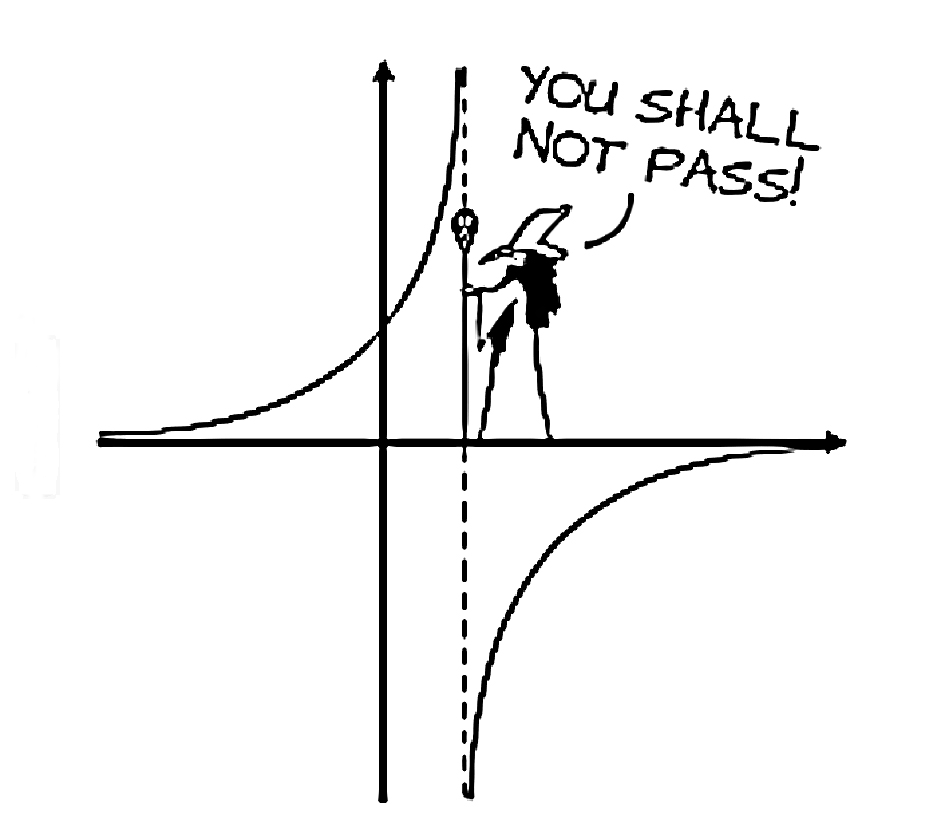
\includegraphics[width=0.8\textwidth]{youshallnotpass}
  \vfill
\end{center}
%\vfill
\vspace*{-2cm}
\begin{singlespace}
\subsection*{Doelstellingen}
Je kan \hfill  {\scriptsize(LP 2005/069, LI 1.3, ET10,11,12,13)}
\begin{itemize}
  \item rationale vergelijkingen van de vorm $\frac{ax+b}{cx+d}=0$ oplossen;
\item aan de hand van het functievoorschrift: een tabel, het domein, de nulwaarden, het tekenverloop en de grafiek bepalen van rationale functies $f(x)=\frac{ax+b}{cx+d}$,
  \item van de grafiek van rationale functies $f(x)=\frac{ax+b}{cx+d}$ het stijgen/dalen, de limietwaarden en het asymptotisch gedrag aflezen,
  \item veranderingen beschrijven en vergelijken met behulp van differentiequotiënten.
  \item problemen met gegeven functioneel verband (rationale functies $f(x)=\frac{ax+b}{cx+d}$) oplossen en deze oplossing interpreteren.
\end{itemize}
\end{singlespace}

\thispagestyle{empty}
\newpage
\thispagestyle{empty}
\tableofcontents
\newpage
\clearpage
\pagenumbering{arabic}
\pagestyle{fancy}
\lhead{}
\fancyhead[RO,LE]{Rationale functies}
\fancyhead[RE,LO]{}

\onehalfspacing

\vspace*{-2cm}
\section*{Inleidende woordzoeker}
Hieronder vind je 18 vragen waarvan je het antwoord in de puzzel moet noteren. Indien je alles juist hebt vind je een wiskundig begrip dat van belang zal zijn in het komende hoofdstuk!

Normaal gezien zou je onderstaande vragen redelijk vlot moeten kunnen oplossen. Soms gaat het om terminologie, soms moet je even een berekening maken. Veel puzzelplezier!

\subsection*{Vragen}

\begin{enumerate}
  \item De verzameling van alle $y$-waarden van een functie.
  \item Los de vergelijking $5x+x=6$ op en noteer het antwoord in woorden.
  \item 0, 1, 2, 3, 4, 5, 6, 7, 8 en 9 zijn \arule{4cm}.
  \item Boven de breukstreep vind je de \arule{4cm}.
  \item Een $x$-waarde waarvoor geldt dat $y$ gelijk is aan nul.
  \item Synoniem voor een lineaire functie.
  \item De verzameling van alle $x$-waarden waarvoor je de $y$-waarde kan berekenen.
  \item Een reële functie is een verzameling van \arule{4cm} reële getallen.
  \item Bepaal de discriminant van de volgende tweedegraadsvergelijking: $2x^2-4x-6=0$.
  \item Het \arule{4cm} van een functie opstellen, betekent dat we nagaan welk teken het beeld $y$ heeft als het argument $x$ het domein doorloopt.
  \item $ax^2+bx+c=0$ is de \arule{4cm} van een tweedegraadsvergelijking.
  \item Breuken behoren tot de verzameling van de \arule{4cm} getallen.
  \item Los de vergelijking $\left(\frac{3}{2}-\frac{2x}{3}\right)-\left(\frac{x}{3}-\frac{3}{2}\right)=1$ op en noteer het antwoord in woorden.
  \item Heeft de functie $f(x)=-\frac{3}{4}x^2+3x$ een absoluut minimum of een absoluut maximum?
  \item Hoe heet het 17de eeuwse zeer symmetrische bouwwerk dat je kan gaan bezoeken in Noord-India?
  \item We spreken van de hellingsgraad van een eerstegraadsfunctie of van de \arule{3cm} van een eerstegraadsfunctie.
  \item Dit moet je berekenen om het aantal oplossingen van een tweedegraadsvergelijking te bepalen.
  \item Bepaal de nulwaarde van deze eerstegraadsfunctie: $y=x-2$.
\end{enumerate}

\subsection*{Woordpuzzel}

\begin{Puzzle}{22}{18}
|{}  |{}  |{}  |{}  |{}  |{}  |{}  |{}  |{}  |{}  |[1] B|   E|   R|   E|   I|   K|.
|{}  |{}  |{}  |{}  |{}  |{}  |{}  |{}  |{}  |   E|[2] E|   N|.
|{}  |{}  |{}  |{}  |   C|   I|   J|   F|   E|   R|[3] S|.
|{}  |{}  |{}  |{}  |{}  |{}  |{}  |{}  |{}  |{}  |[4] T|   E|   L|   L|   E|   R|.
|{}  |{}  |{}  |{}  |{}  |{}  |   N|   U|   L|   W|[5] A|   A|   R|   D|   E|.
|{}  |   E|   E|   R|   S|   T|   E|   G|   R|   A|[6] A|   D|   S|   F|   U|   N|   C|   T|   I|   E|.
|{}  |{}  |{}  |{}  |{}  |   D|   O|   M|   E|   I|[7] N|.
|{}  |{}  |{}  |{}  |   K|   O|   P|   P|   E|   L|[8] S|.
|{}  |{}  |{}  |{}  |{}  |{}  |{}  |{}  |{}  |{}  |[9] V|   I|   E|   R|   E|   N|   Z|   E|   S|   T|   I|   G|.
|{}  |   T|   E|   K|   E|   N|   V|   E|   R|   L|[10]O|   O|   P|.
|   S|   T|   A|   N|   D|   A|   A|   R|   D|   V|[11]O|   R|   M|.
|{}  |{}  |{}  |{}  |{}  |{}  |{}  |{}  |{}  |{}  |[12]R|   A|   T|   I|   O|   N|   A|   L|   E|.
|{}  |{}  |{}  |{}  |{}  |{}  |{}  |{}  |{}  |   T|[13]W|   E|   E|.
|{}  |{}  |{}  |{}  |{}  |{}  |{}  |{}  |{}  |   M|[14]A|   X|   I|   M|   U|   M|.
|{}  |{}  |{}  |   T|   A|   J|{}  |   M|   A|   H|[15]A|   L|.
|{}  |{}  |{}  |{}  |{}  |{}  |{}  |{}  |{}  |{}  |[16]R|   I|   C|   O|.
|{}  |{}  |{}  |{}  |{}  |{}  |{}  |{}  |{}  |{}  |[17]D|   I|   S|   C|   R|   I|   M|   I|   N|   A|   N|   T|.
|{}  |{}  |{}  |{}  |{}  |{}  |{}  |{}  |   T|   W|[18]E|   E|.
\end{Puzzle}

\subsection*{Oplossing}
\begin{wrapfigure}[0]{r}{0.25\textwidth}
  \vspace*{-2cm}
  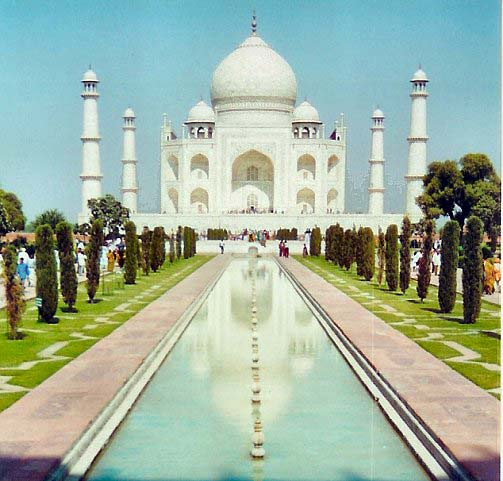
\includegraphics[width=0.25\textwidth]{taj-mahal}
\end{wrapfigure}
Het gevonden wiskundewoord is \arule{5cm}.

\pagebreak

\end{theorie}

\section{Rationale vergelijkingen}

\begin{theorie}

\subsection{Definitie}

\begin{mdframed}
Een {\bf rationale vergelijking} is een vergelijking van de vorm
$$\dfrac{p(x)}{q(x)}=0$$
met $p(x)$ en $q(x)$ veeltermen.
\end{mdframed}

Het randgeval waarbij $q(x)=c$ met $c$ een constante $\in \mathbb{R}$ is dan ook een veeltermvergelijking. Veeltermvergelijkingen werden reeds in een vorig hoofdstuk besproken.

\subsection{Standaardvorm}

\begin{mdframed}
We noemen de rationale vergelijking
$$\dfrac{ax+b}{cx+d}=0$$
de {\bf standaardvorm}.
\end{mdframed}
Dit is een simpele vorm van rationale vergelijkingen. De teller en de noemer zijn beide eerstegraadsveeltermen. Wij zullen deze in detail bespreken, daarnaast zullen we ook rationale vergelijkingen zien waarbij de graad van teller en noemer hoger kan zijn.

\end{theorie}

\begin{oefening}
Zijn de volgende vergelijkingen rationale vergelijkingen? Herleid de rationale vergelijkingen ook steeds op 0.
\begin{multicols}{2}
\begin{enumerate}[(a)]
  \itemsep1em
  \item $\dfrac{x+3}{2x-6}=0$
  \item $\dfrac{2x-1}{x}+\dfrac{3}{2x}=0$
  \item $\dfrac{3x+2}{\sqrt{x}}=0$
  \item $\dfrac{8x-6}{2}=0$
  \item $\dfrac{1}{x^2-x-1}=0$
  \item $\dfrac{2x}{\sqrt{x}-1}+3=0$
  \item $\dfrac{3x+1}{2x-4}=\dfrac{3x+1}{2x+4}$
  \item $\dfrac{3x+2}{\frac{3x-2}{x+1}}=0$
  \item $\dfrac{4x^4+3x^3+2x^2+x}{x}=0$
  \item $\dfrac{\sqrt{x^2+2x+1}}{x-1}=0$
\end{enumerate}
\end{multicols}
\end{oefening}

\begin{theorie}

\subsection{Bestaansvoorwaarde}
Als we vergelijkingen oplossen, dan eisen we dat de gevonden oplossingen wel degelijk in de vergelijking ingevuld kunnen worden. Bij rationale vergelijkingen zullen we daarom eisen dat de noemer geen nul wordt. Deze eis is de {\bf bestaansvoorwaarde} of kort {\bf BV}. Voor onze eenvoudige standaardvorm
$$\dfrac{ax+b}{cx+d}=0$$
wordt dit
\begin{align*}
  \mbox{BV: } cx+d &\neq 0\\
                cx &\neq -d\\
                 x &\neq -\dfrac{d}{c}
\end{align*}


\subsection{Voorbeelden}

Los op in $\mathbb{R}$:
$$\frac{2x+3}{x+3} = 0$$
$$\mbox{BV: }x\neq -3 \qquad V=\{-\dfrac{3}{2}\}$$


Los op in $\mathbb{R}$:
$$\frac{1}{x+2}+\frac{4}{3x-4}=1$$
$$\mbox{BV: }x\neq -2 \vee x\neq \dfrac{4}{3} \qquad V=\{3,-\dfrac{4}{3}\}$$

Los op in $\mathbb{R}$:
$$\frac{x^2-4}{x+2}=0$$
$$\mbox{BV: }x\neq -2 \qquad V=\{2\}$$

\subsection{Werkwijze}
\begin{enumerate}[(1)]
  \item Je herleidt de gegeven vergelijking op nul.
  \item Je stelt de bestaansvoorwaarde op.
  \item Je stelt de teller gelijk aan nul en lost deze op.
  \item Je schrijft de oplossingsverzameling $V$, hier komen alle oplossingen in als ze voldoen aan de bestaansvoorwaarde.
\end{enumerate}

\end{theorie}

\begin{oefening}
Los op in $\mathbb{R}$:
\begin{multicols}{2}
\begin{enumerate}[(a)]
  \itemsep1em
  \item $\dfrac{x-3}{x+2}=0$
  \item $\dfrac{2}{-2x+3}=0$
  \item $\dfrac{-x}{5-x}=0$
  \item $\dfrac{-2x-2}{-x+2}=0$
  \item $\dfrac{x-2}{-x+2}=0$
  \item $\dfrac{(2x+2)^2-4x^2}{x-2}=0$
  \item $\dfrac{(x-4)^2-x^2}{x-2}=0$
  \item $\dfrac{x^2+(2-x)(2+x)}{-2x+4}=0$
\end{enumerate}
\end{multicols}
\end{oefening}

\begin{oefening}
Los op in $\mathbb{R}$:
\begin{multicols}{2}
\begin{enumerate}[(a)]
  \itemsep1em
  \item $\dfrac{1}{x-2}+\dfrac{1}{x+4}=0$
  \item $\dfrac{2}{x+3}+\dfrac{3}{2x-2}=0$
  \item $\dfrac{x-2}{x-4}-\dfrac{1}{x+4}=0$
  \item $\dfrac{x^2-1}{(x+1)^2}=0$
  \item $\dfrac{x+2}{x-7}+2=\dfrac{3x+1}{x-3}$
  \item $\dfrac{1}{x}-\dfrac{5}{2x-3}=\dfrac{x+1}{2x^2-3x}$
\end{enumerate}
\end{multicols}
\end{oefening}

\begin{oefening}  % extra oefeningen door Staelens
Los de volgende rationale vergelijkingen op:
\begin{enumerate}[(a)]
  \itemsep1em
  \item $\dfrac{x-3}{x+2}=0$
  \item $\dfrac{2}{x-5}=1$
  \item $\dfrac{x}{x-5}+2=\dfrac{5}{x-5}$
  \item $\dfrac{x-1}{x+1}=3-\dfrac{2}{x+1}$
  \item $\dfrac{2}{x}+3=\dfrac{4}{x}$
\end{enumerate}
\end{oefening}

\pagebreak
\section{Rationale functies}

\begin{theorie}

\subsection{Definities}

Wanneer we een functie $f(x)$ hebben waarbij er een breuk is met in de noemer een onbepaalde $x$, zullen we van een rationale functie spreken.

\paragraph*{Definitie}
\begin{mdframed}
Een {\bf rationale functie} is een reële functie met een voorschrift van de vorm

$$f(x)=\dfrac{p(x)}{q(x)}$$

waarbij $p(x)$ en $q(x)$ veeltermen zijn.
\end{mdframed}

We zullen voornamelijk rationale functies behandelen waarbij:
\begin{itemize}
  \item de teller en noemer van de eerste graad zijn;
  \item de nulwaarde van teller en van noemer verschillend zijn.
\end{itemize}
Deze functies worden homografische functies genoemd:

\paragraph*{Definitie}
\begin{mdframed}
Een {\bf homografische functie} is een functie van de vorm
$$f(x)=\dfrac{ax+b}{cx+d}$$
met $c\neq 0$ en $a\cdot d\neq b\cdot c$.
\end{mdframed}

\end{theorie}

\begin{oefening}
Zijn volgende functies rationale functies? Zijn ze homografische functies?
\begin{multicols}{2}
\begin{enumerate}[(a)]
  \itemsep1em
  \item $f(x)=\dfrac{5x-3}{x-2}$
  \item $f(x)=\dfrac{4x-4}{x-1}$
  \item $f(x)=\dfrac{5}{x-3}$
  \item $f(x)=\dfrac{2x-4}{x-2}$
  \item $f(x)=\dfrac{x^2-4}{x+4}$
  \item $f(x)=\dfrac{4x^2-8}{2}$
  \item $f(x)=\dfrac{x^2-4}{x-4}$
  \item $f(x)=\dfrac{1+4x}{x}+\dfrac{3x-6}{x}$
  \item $f(x)=\dfrac{1+x^2}{\sqrt{x}+3}$
  \item $f(x)=\dfrac{3x^3-x^2-2}{x^4+x^3-x^2-1}$
\end{enumerate}
\end{multicols}
\end{oefening}

\begin{oefening}
Bespreek:
\begin{enumerate}[(a)]
  \item Zijn alle rationale functies homografische functies?
  \item Zijn alle homografische functies rationale functies?
\end{enumerate}
\end{oefening}

\begin{theorie}

Om de nulwaarden van een rationale functie te vinden zullen we de $y$-waarde gelijk stellen aan $0$. We lossen dus een rationale vergelijking op. Daarom krijgen we de volgende eigenschap:

\paragraph*{Eigenschap}
\begin{mdframed}
De {\bf nulwaarde} van een rationale functie is de nulwaarde van de teller die geen nulwaarde is van de noemer.
\end{mdframed}

In de nulwaarde van de noemer heeft de rationale functie uiteraard geen functiewaarde. Zulk een waarde zullen we een pool noemen:

\paragraph*{Definitie}
\begin{mdframed}
Een nulwaarde van de noemer van een rationale functie noemen we een {\bf pool} van de rationale functie.
\end{mdframed}

\end{theorie}

\begin{oefening}
Bepaal de polen en de nulwaarden van de volgende functies:
\begin{multicols}{2}
\begin{enumerate}[(a)]
  \itemsep1em
  \item $f(x)=\dfrac{5x-3}{x-2}$
  \item $f(x)=\dfrac{4x-4}{x-1}$
  \item $f(x)=\dfrac{5}{x-3}$
  \item $f(x)=\dfrac{2x-4}{x-2}$
  \item $f(x)=\dfrac{x^2-4}{x+2}$
  \item $f(x)=\dfrac{x^2-4}{x-2}$
  \item $f(x)=\dfrac{1+4x}{x}+\dfrac{3x-6}{x}$
  \item $f(x)=\dfrac{3x^3-x^2-2}{x^4+x^3-x^2-1}$
  \item $f(x)=1+\dfrac{2x+6}{x}$
  \item $f(x)=\dfrac{3x}{4x+1}+\dfrac{1}{x}$
  \item $f(x)=\dfrac{3}{5-x}+\dfrac{2}{4-x}-\dfrac{5}{3-x}$
  \item $f(x)=\dfrac{x+2}{x-7}+2-\dfrac{3x+1}{x-3}$
\end{enumerate}
\end{multicols}\end{oefening}

\begin{oefening}
\begin{enumerate}[(a)]
  \item Hoeveel polen zal een rationale functie maximaal hebben?
  \item Hoeveel nulwaarden zal een rationale functie maximaal hebben?
  \item Kan een rationale functie, waarvan de noemer zeker een onbepaalde $x$ bevat, nul polen hebben? Geef een voorbeeld.
  \item Kan een rationale functie geen nulwaarden hebben? Geef een voorbeeld.
\end{enumerate}
\end{oefening}

\begin{theorie}

\pagebreak
\subsection{Bespreken van een rationale functie}
\subsubsection*{Voorbeeld}
We bespreken de eenvoudige homografische functie
$$f(x)=\frac{x-1}{x+1}$$

We wensen zo snel mogelijk de grafiek te tekenen. Hiervoor zullen we een functiewaardentabel opstellen. We moeten echter wel eerst nog weten rond welk interval we de functiewaardentabel zullen bepalen. Hiervoor bepalen we eerste een aantal interessante waarden:

\begin{itemize}
  \item nulwaarde noemer: $x=-1$\\
  Dit is een pool van de rationale functie, deze waarde behoort uiteraard niet tot het domein.
  \item nulwaarde teller: $x=1$\\
  Aangezien de nulwaarde van de teler geen pool is, is het ook een nulwaarde van de functie:
  \item nulwaarde functie: $x=1$\\  
\end{itemize}

Met deze informatie hebben we dus reeds het domein van de functie gevonden, dit is namelijk alle reële getallen zonder de polen:
\begin{itemize}
  \item $\dom f= \mathbb{R}\setminus \{-1\}$
\end{itemize}

We kunnen nu het tekenverloop van de functie bepalen door afzonderlijk van teller en van noemer het tekenverloop te bepalen. Aangezien teller wordt gedeeld door de noemer kunnen we het teken van de functie eenvoudig afleiden met de regel: {\em Een oneven aantal min geeft min}. Een verticaal streepje wordt gebruikt waar de functie geen beeld heeft:

\begin{itemize}
  \item tekenverloop:
  \begin{center}
    \begin{tabular}{c|ccccccc}
    $x$ & $-\infty$ & & -1 & & 1 & & $+\infty$\\   
    \hline
    $x-1$ & & - &   & - & 0 & + & \\
    $x+1$ & & - & 0 & + &   & + & \\
    \hline
    $f(x)=y$ & & + & $|$ & - & 0 & +
    \end{tabular}
  \end{center}
\end{itemize}

We zorgen nu dat er voldoende waarden voor, tussen en na de bijzondere $x$-waarden $-1$ en $1$ komen in onze functiewaardentabel:

\begin{itemize}
\item Functiewaardentabel:
\begin{center}
\hspace*{-2cm}
\begin{tabular}{c|cccccccccccccccc}
  $x$ & -5 & -4 & -3 & -2 & $-\frac{3}{2}$ & -1 & $-\frac{1}{2}$ & $-\frac{1}{3}$ & 0 & 1 & 2 & 3 & 4\\
  \hline
  $f(x)$\\
\end{tabular}
\end{center}
\end{itemize}

We hebben nu zeker voldoende punten om de grafiek te tekenen. We verbinden de punten met een vloeiende lijn, enkel aan de pool $x=-1$ moeten we even de grafiek onderbreken om de pen op te heffen en te verplaatsen naar het nieuwe punt. Het is ook aan te raden om de gebieden waar de grafiek positief en negatief (zie tekenverloop) is aan te duiden, zoals op onderstaande grafiek.

\begin{itemize}
  \item Grafiek:
\end{itemize}

\begin{center}
\definecolor{aqaqaq}{rgb}{0.6274509803921569,0.6274509803921569,0.6274509803921569}
\begin{tikzpicture}[line cap=round,line join=round,>=triangle 45,x=1.0cm,y=1.0cm]
\draw[->,color=black] (-5.14,0.) -- (4.16,0.);
\foreach \x in {-5.,-4.,-3.,-2.,-1.,1.,2.,3.,4.}
\draw[shift={(\x,0)},color=black] (0pt,2pt) -- (0pt,-2pt) node[below] {\footnotesize $\x$};
\draw[->,color=black] (0.,-4.16) -- (0.,5.32);
\foreach \y in {-4.,-3.,-2.,-1.,1.,2.,3.,4.,5.}
\draw[shift={(0,\y)},color=black] (2pt,0pt) -- (-2pt,0pt) node[left] {\footnotesize $\y$};
\draw[color=black] (0pt,-10pt) node[right] {\footnotesize $0$};
\clip(-5.14,-4.16) rectangle (4.16,5.32);
\fill[line width=0.pt,color=aqaqaq,fill=aqaqaq,fill opacity=0.35] (-1.,0.) -- (-8.,0.) -- (-8.02,7.3) -- (-1.,7.3) -- cycle;
\fill[line width=0.pt,color=aqaqaq,fill=aqaqaq,fill opacity=0.35] (-1.,0.) -- (1.,0.) -- (1.,-6.) -- (-1.,-6.) -- cycle;
\fill[line width=0.pt,color=aqaqaq,fill=aqaqaq,fill opacity=0.35] (1.,0.) -- (7.24,0.) -- (7.26,7.28) -- (1.,7.26) -- cycle;
\draw[line width=2.pt,smooth,samples=100,domain=-5.1:-1.01] plot(\x,{((\x)-1.0)/((\x)+1.0)});
\draw[line width=2.pt,smooth,samples=100,domain=-0.99:4.1] plot(\x,{((\x)-1.0)/((\x)+1.0)});
\draw (3.02,1.16) node[anchor=north west] {f};
\draw (-0.42,-0.26) node[anchor=north west] {-};
\draw (-2.36,1.16) node[anchor=north west] {+};
\draw (2.2,1.08) node[anchor=north west] {+};
\begin{scriptsize}
\draw[color=black] (-8.08,1.16) node {$f$};
\end{scriptsize}
\end{tikzpicture}
\end{center}

Een grafiek van deze vorm noemen we een {\bf hyperbool}. Homografische functies zullen altijd aanleiding geven tot een hyperbool.

Met de grafiek nu redelijk nauwkeurig getekend is het eenvoudig om het stijgen en dalen af te lezen:

\begin{itemize}
  \item Stijgen\&dalen:
  \begin{center}
    \begin{tabular}{c|ccccc}
      $x$ & $-\infty$ & & $-1$ & & $+\infty$\\
      \hline
      $f(x)=y$ & & $\nearrow$ & $|$ & $\nearrow$ &
    \end{tabular}
  \end{center}
\end{itemize}

We zien op de grafiek dat als we de $x$-waarde in de richting van $-\infty$ laten naderen, dat de $y$-waarde waarde dan steeds dichter naar $1$ zal gaan. Analoog als we de $x$-waarde dichter en dichter naar $+\infty$ laten gaan, dat de $y$-waarde dan steeds dichter naar $1$ zal gaan.

Ook de $x$-waarde $x=-1$ is bijzonder. Als we deze op de $x$-as naderen van links naar rechts (dus van kleiner dan $-1$ naar $-1$) dan zal de $y$-waarde steeds dichter bij $+\infty$ naderen. Als we aan de andere kant, van rechts naar links (dus van groter dan $-1$ naar $-1$) gaan, dan zal de $y$-waarde steeds dichter bij $-\infty$ naderen.

We schrijven dit kort als:

\begin{itemize}
  \item $\displaystyle\lim_{x\to -\infty}=1$
  \item $\displaystyle\lim_{x\to +\infty}=1$
  \item $\displaystyle\lim_{x\underset{<}{\to} -1}=+\infty$
  \item $\displaystyle\lim_{x\underset{>}{\to} -1}=+\infty$
\end{itemize}

We bepalen nu ook nog de rechten waarnaar de grafiek (in ons geval een hyperbool) steeds dichter naar zal naderen. Deze rechten noemen we asymptoten. Meer specifiek is de rechte met vergelijking $y=1$ de horizontale asymptoot van de hyperbool. De rechte met vergelijking $x=-1$ is de verticale asymptoot van de hyperbool. We noteren kort:

\begin{itemize}
  \item H.A. : $y=1$
  \item V.A. : $x=-1$
\end{itemize}

We verbeteren nu nog onze grafiek door ook de asymptoten (in een ander kleur of in stippellijn) hier op aan te duiden:

\begin{center}
\begin{tikzpicture}[scale=0.9,line cap=round,line join=round,>=triangle 45,x=1.0cm,y=1.0cm]
\draw[->,color=black] (-7.36,0.) -- (7.36,0.);
\foreach \x in {-7.,-6.,-5.,-4.,-3.,-2.,-1.,1.,2.,3.,4.,5.,6.,7.}
\draw[shift={(\x,0)},color=black] (0pt,2pt) -- (0pt,-2pt) node[below] {\footnotesize $\x$};
\draw[->,color=black] (0.,-5.5) -- (0.,6.76);
\foreach \y in {-5.,-4.,-3.,-2.,-1.,1.,2.,3.,4.,5.,6.}
\draw[shift={(0,\y)},color=black] (2pt,0pt) -- (-2pt,0pt) node[left] {\footnotesize $\y$};
\draw[color=black] (0pt,-10pt) node[right] {\footnotesize $0$};
\clip(-7.36,-5.5) rectangle (7.36,6.76);
\draw[line width=2.pt,smooth,samples=100,domain=-7.3:-1.01] plot(\x,{((\x)-1.0)/((\x)+1.0)});
\draw[line width=2.pt,smooth,samples=100,domain=-0.99:7.36] plot(\x,{((\x)-1.0)/((\x)+1.0)});
\draw (-3.9,2.44) node[anchor=north west] {$f$};
\draw [line width=1.2pt,dash pattern=on 2pt off 2pt] (-1.,-5.5) -- (-1.,6.76);
\draw [line width=1.2pt,dash pattern=on 2pt off 2pt,domain=-7.36:7.36] plot(\x,{(--1.-0.*\x)/1.});
\draw (-4,-2.68) node[anchor=north west] {VA: $x=-1$};
\draw (3.78,1.8) node[anchor=north west] {HA: $y=1$};
\end{tikzpicture}
\end{center}


\subsubsection*{Werkwijze}

%Bij het bespreken van een rationale functie wil je zo snel mogelijk de grafiek kunnen maken. Hiervoor heb je de functiewaardentabel van de functie nodig. Het probleem is nu om te weten van waar tot waar we de functiewaardentabel moeten maken en met welke stapjes we moeten gaan. In je functiewaardentabel wens je zeker alle interessante waarden te vinden, en deze vind je bij een functie meestal rond de nulwaarden. Daarom ga je als volgt te werk:\\

Schrijf de functie als
$$f(x)=\dfrac{T(x)}{N(x)}$$
\begin{enumerate}
\singlespacing
%\small
  \item Bepaal de nulwaarden
  \begin{description}
    \item[nulwaarde noemer] (nulw $N$) Hier heeft de functie geen beeld, we zeggen dat de functie een pool heeft op deze $x$-waarde.
    \item[nulwaarde teller] (nulw $T$) Hier vinden we mogelijks de nulwaarden van de functie zelf, op voorwaarde dat de functie daar geen pool heeft.
    \item[nulwaarde functie] (nulw $f$) Alle nulwaarden van de teller die geen nulwaarde van de noemer zijn.
  \end{description}
  \item Bepaal het domein: dit is nu de verzameling van de reële getallen zonder de polen
  $$\mbox{dom }f = \mathbb{R}\setminus \{\mbox{nulw} N\}$$
  \item Maak het tekenverloop van de functie. Maak hiervoor een tekenschema met vier rijen.
  \begin{description}
    \item[rij 1:] $x$ De rij met alle $x$-waarden, hier komen alle nulwaarden, zowel van teller als van noemer.
    \item[rij 2:] $T$ De rij met het tekenverloop van de teller. Duid op de plaats van de nulwaarde van de teller een nul aan, bepaal tussen de nulwaarden het teken van de teller.
    \item[rij 3:] $N$ De rij met het tekenverloop van de noemer. Duid op de plaats van de nulwaarde van de noemer een nul aan, bepaal tussen de nulwaarden het teken van de noemer.
    \item[rij 4:] $f$ De rij met het tekenverloop van de functie $f$ zelf. Hiervoor ga je als volgt te werk: kijk kolom per kolom naar het aantal minnen, een oneven aantal minnen geeft je opnieuw een min, een even aantal minnen geeft je een plus, een nul in de noemer geeft je een verticaal streepje, als er enkel een nul in de teller staat mag je een nul schrijven.
  \end{description}
  \item Maak de functiewaardentabel van $f$, deze moet zeker alle nulwaarden van teller en noemer bevatten en een aantal waarden links en rechts hiervan. Neem ook voldoende tussenliggende waarden.
  \item Maak de grafiek van de functie met behulp van alle info die je nu hebt verzameld.
  \item Bepaal de limietwaarden en bijgevolg ook de asymptoten, gebruik de gemaakte grafiek of:
  \begin{itemize}
  \scriptsize
    \item $x\to-\infty$: Gebruik het rekentoestel om de $y$-waarde te bepalen waarnaar de functie gaat voor heel kleine waarden van $x$.
    \item $x\to+\infty$: Gebruik het rekentoestel om de $y$-waarde te bepalen waarnaar de functie gaat voor heel grote waarden van $x$.
    \item $x$ nabij de polen: Je kan zien of ze komende van links/recht naar $+\infty$ of naar $-\infty$ gaan.
  \end{itemize}
  %\item Bepaal aan de hand van de grafiek het bereik. Vaak zal er bij een horizontale asymptoot geen beeld zijn van de de functie.
  \item Bepaal ook nog het stijgen, dalen en eventueel de extrema.
  %\item Bereken eventueel ook nog de differentiequotiënten.
\end{enumerate}

\end{theorie}

\begin{oefening}
Bespreek volgende homografische functies:
\begin{multicols}{2}
\begin{enumerate}[(a)]
  \itemsep1em
  \item $f(x)=\dfrac{2x+3}{x+3}$
  \item $f(x)=\dfrac{-x}{5-x}$
  \item $f(x)=\dfrac{2}{-2x+3}$
  \item $f(x)=\dfrac{-2x-2}{-x+2}$
  \item $f(x)=\dfrac{x}{x-3}$
  \item $f(x)=\dfrac{1}{x-2}+\dfrac{3}{x-2}$
  \item $f(x)=\dfrac{5x-3}{x-2}$
  \item $f(x)=\dfrac{4x-4}{x-1}$
  \item $f(x)=\dfrac{5}{x-3}$
  \item $f(x)=\dfrac{2x-4}{x-2}$
  \item $f(x)=\dfrac{x^2-4}{x+2}$
  \item $f(x)=\dfrac{x^2-4}{x-2}$
  \item $f(x)=\dfrac{1+4x}{x}+\dfrac{3x-6}{x}$
  \item $f(x)=1+\dfrac{2x+6}{x}$
\end{enumerate}
\end{multicols}
\end{oefening}

\begin{oefening}*
Bespreek volgende rationale functies:
\begin{multicols}{2}
\begin{enumerate}[(a)]
  \itemsep1em
  \item $f(x)=\dfrac{x^2-4}{x^2-6x}$
  \item $f(x)=\dfrac{x^2+2x+1}{x+1}$
  \item $f(x)=\left(\dfrac{x-2}{x+2}\right)^2$
  \item $f(x)=\dfrac{3x}{4x+1}+\dfrac{1}{x}$
  \item $f(x)=\dfrac{3x^3-x^2-2}{x^4+x^3-x^2-1}$
  \item $f(x)=\dfrac{3}{5-x}+\dfrac{2}{4-x}-\dfrac{5}{3-x}$
  \item $f(x)=\dfrac{x+2}{x-7}+2-\dfrac{3x+1}{x-3}$
\end{enumerate}
\end{multicols}
\end{oefening}

\pagebreak
\section{Differentiequotiënt van een rationale functie}

\begin{theorie}

\subsection{Voorbeeld}

Beschouw de homografische functie
$$f(x)=\dfrac{4x-7}{x-1}$$

Homografische functies zijn ofwel stijgend, ofwel dalend in hun domein. Zonder de grafiek te tekenen kunnen we dit heel snel bepalen door de functiewaarde in twee nabijgelegen punten te bepalen en het verschil geeft dan de helling:

\begin{itemize}
  \item $f(2)=1$ en $f(2.5)=2$ $\Rightarrow$ op het interval $[2,2.5]$ stijgt de functie $1$ eenheid
  \item $f(3)=2.5$ en $f(7)=3.5$ $\Rightarrow$ op het interval $[3,7]$ stijgt de functie $1$ eenheid
\end{itemize}

We maken de grafiek en duiden er beide situaties op aan:

\begin{center}
\definecolor{ffqqqq}{rgb}{1,0,0}
\definecolor{uququq}{rgb}{0.25,0.25,0.25}
\begin{tikzpicture}[line cap=round,line join=round,>=triangle 45,x=1.0cm,y=1.0cm]
\draw[->,color=black] (-2.44,0) -- (10.68,0);
\foreach \x in {-2,2,4,6,8,10}
\draw[shift={(\x,0)},color=black] (0pt,2pt) -- (0pt,-2pt) node[below] {\footnotesize $\x$};
\draw[->,color=black] (0,-2.55) -- (0,8.46);
\foreach \y in {-2,2,4,6,8}
\draw[shift={(0,\y)},color=black] (2pt,0pt) -- (-2pt,0pt) node[left] {\footnotesize $\y$};
\draw[color=black] (0pt,-10pt) node[right] {\footnotesize $0$};
\clip(-2.44,-2.55) rectangle (10.68,8.46);
\draw[line width=1.4pt, smooth,samples=100,domain=-2.4:0.9] plot(\x,{(4*(\x)-7)/((\x)-1)});
\draw[line width=1.4pt, smooth,samples=100,domain=1.1:10.6] plot(\x,{(4*(\x)-7)/((\x)-1)});
\draw(8.01,-8.36) -- (10.85,-8.36);
\draw(8.01,-9.41) -- (10.85,-9.41);
\draw [color=ffqqqq,domain=-2.44:10.68] plot(\x,{(-1.5--1*\x)/0.5});
\draw [color=ffqqqq,domain=-2.44:10.68] plot(\x,{(--7--1*\x)/4});
\begin{scriptsize}
\fill [color=black] (8.01,-8.36) circle (1.5pt);
\draw[color=black] (8.18,-7.84) node {$a = 2$};
\fill [color=black] (8.24,-9.41) circle (1.5pt);
\draw[color=black] (8.58,-8.9) node {$b = 2.5$};
\fill [color=uququq] (2,1) circle (1.5pt);
\draw[color=uququq] (1.52,1.2) node {$A$};
\fill [color=uququq] (2.5,2) circle (1.5pt);
\draw[color=uququq] (2.09,2.6) node {$B$};
\fill [color=uququq] (3,2.5) circle (1.5pt);
\draw[color=uququq] (3.17,2.17) node {$C$};
\fill [color=uququq] (7,3.5) circle (1.5pt);
\draw[color=uququq] (7.04,3.14) node {$D$};
\end{scriptsize}
\end{tikzpicture}
\end{center}

We zien dat, door rekening te houden met de afstand van het interval, dat we ook informatie krijgen over hoe steil dat de functie gemiddeld stijgt op het interval:
\begin{itemize}
  \item $\dfrac{f(2.5)-f(2)}{2.5-2}=\dfrac{2-1}{0.5}=2$ $\Rightarrow$ op $[2, 2.5]$ stijgt de functie gemiddeld 2 eenheden
  \item $\dfrac{f(7)-f(3)}{7-3}=\dfrac{3.5-2.5}{4}=0.25$ $\Rightarrow$ op $[2, 2.5]$ stijgt de functie gemiddeld 0.25 eenheden
\end{itemize}

We noemen dit de gemiddelde verandering van een functie in een interval en berekenen dit met de differentiequotiënt.

We kunnen de differentiequotiënt ook gebruiken om aan te tonen dat homografische functies een horizontale asymptoot hebben:
\begin{itemize}
  \item $f(1000)=3.9969$ en $f(2000)=3.9984$
  \item $\dfrac{f(2000)-f(1000)}{2000-1000}=\dfrac{3.9984-3.9969}{1000}=\dfrac{0.0015}{1000}=0.0000015$
\end{itemize}
We merken dat de gemiddelde stijging heel klein, maar nog steeds positief is.

Wat gebeurt er als we de differentiequotiënt berekenen voor een steeds kleiner wordend interval? We krijgen niet meer de gemiddelde stijging, maar de stijging in één enkel punt! Dit noemen we de ogenblikkelijke stijging en deze geeft ons de helling van de raaklijn aan de functie.

Merk verder op dat de differentiequotiënt berekenen in een interval waar er een pool ligt zinloos is!

\subsection{Definitie}
\paragraph{Differentiequotiënt}
\begin{mdframed}
het differentiequotiënt $\dfrac{\Delta y}{\Delta x}$ van een functie $f$ voor een interval $[a, b]$ is de gemiddelde verandering van deze functie in het interval. We bereken
$$\dfrac{\Delta y}{\Delta x}=\dfrac{f(b)-f(a)}{b-a}$$
\end{mdframed}

We spreken af dat we geen differentiequotiënt kunnen berekenen in een interval $[a,b]$ dat een verticale asymptoot bevat. Wij zullen ons beperken tot homografische functies. Bij homografische functies mag de pool dus niet in het interval liggen.

Als we in het interval $[a,b]$ de grens $b$ naar $a$ laten gaan, dan krijgen we de helling van de raaklijn aan de functie $f$ in $a$. We krijgen met andere woorden de ogenblikkelijke verandering in $a$. We noteren dit als de afgeleide waarde van $f$ in $a$:
$$f'(a)=\lim_{b\to a}\dfrac{f(b)-f(a)}{b-a}$$

\pagebreak
\subsection{Oefeningen}

\end{theorie}

\begin{oefening}
Bepaal voor de volgende functies het differentiequotiënt in het interval $[1,3]$ en duid de koorde aan op de functies.\\
\begin{multicols}{2}
\begin{enumerate}[(a)]
  \itemsep1em
  \item $f(x)=\dfrac{2x+3}{x+3}$
  \item $f(x)=\dfrac{-x}{5-x}$
  \item $f(x)=\dfrac{2}{-2x+3}$
  \item $f(x)=\dfrac{-2x-2}{-x+2}$
  \item $f(x)=\dfrac{x}{x-3}$
  \item $f(x)=\dfrac{1}{x-2}+\dfrac{3}{x-2}$
\end{enumerate}
\end{multicols}
\end{oefening}

\begin{oefening}
Bepaal voor\\
\begin{enumerate}[(a)]
  \itemsep1em
  \item $f(x)=\dfrac{x^2}{1-x}+x$\\
  \begin{itemize}
    \item de differentiequotiënt in $[-2,0.5]$
    \item de differentiequotiënt in $[0.5, 2]$
  \end{itemize}
  \item $f(x)=\dfrac{1}{x-2}-\dfrac{1}{x+2}$\\
  \begin{itemize}
    \item de verticale asymptoten
    \item de differentiequotiënt in $[-1,0]$, $[0,1]$ en $[-1,1]$
  \end{itemize}
  \item $f(x)=\dfrac{2}{x}-2$\\
  \begin{itemize}
    \item de verticale asymptoten
    \item de differentiequotiënt in $[-2,-1]$, $[-1,0]$ en $[0,1]$
  \end{itemize}
\end{enumerate}
\end{oefening}

\begin{oefening}
Beschouw de functie $f(x)=\dfrac{3x}{2x-1}$
\begin{enumerate}[(a)]
  \item Bepaal de verticale asymptoten.
  \item Bepaal de differentiequotiënt in de intervallen $[-3,-2]$; $[-1,0]$; $[0,1]$ en $[1,2]$.
  \item Waarom hebben zijn differentiequotiënten in de intervallen $[-1,0]$ en $[1,2]$ gelijk?
  \item Bepaal de differentiequotiënt in het interval $[10000, 100000]$, wat merk je?
\end{enumerate}
\end{oefening}

\begin{oefening}
\begin{enumerate}[(a)]
  \item Bepaal de differentiequotiënt in het interval $[-8,-2]$ van de functie waarvan de grafiek hieronder is weergegeven.
\begin{center}
\definecolor{cqcqcq}{rgb}{0.75,0.75,0.75}
\begin{tikzpicture}[scale=0.6,line cap=round,line join=round,>=triangle 45,x=1.0cm,y=1.0cm]
\draw [color=cqcqcq,dash pattern=on 2pt off 2pt, xstep=2.0cm,ystep=2.0cm] (-10.39,-3.3) grid (11.47,7);
\draw[->,color=black] (-10.39,0) -- (11.47,0);
\foreach \x in {-10,-8,-6,-4,-2,2,4,6,8,10}
\draw[shift={(\x,0)},color=black] (0pt,2pt) -- (0pt,-2pt) node[below] {\footnotesize $\x$};
\draw[->,color=black] (0,-3.3) -- (0,7);
\foreach \y in {-2,2,4,6}
\draw[shift={(0,\y)},color=black] (2pt,0pt) -- (-2pt,0pt) node[left] {\footnotesize $\y$};
\draw[color=black] (0pt,-10pt) node[right] {\footnotesize $0$};
\clip(-10.39,-3.3) rectangle (11.47,7);
\draw[line width=2.4pt, smooth,samples=100,domain=-10.3:-0.6] plot(\x,{(3*(\x)-6)/(2*(\x)+1)});
\draw[line width=2.4pt, smooth,samples=100,domain=-0.4:11.4] plot(\x,{(3*(\x)-6)/(2*(\x)+1)});
\end{tikzpicture}
\end{center}
  \item Bepaal de differentiequotiënt in het interval $[1,3]$ van de functie waarvan de grafiek hieronder is weergegeven.
\begin{center}
\definecolor{cqcqcq}{rgb}{0.75,0.75,0.75}
\begin{tikzpicture}[scale=0.9,line cap=round,line join=round,>=triangle 45,x=1.0cm,y=1.0cm]
\draw [color=cqcqcq,dash pattern=on 1pt off 1pt, xstep=1.0cm,ystep=1.0cm] (-8.54,-1.82) grid (6.39,5.22);
\draw[->,color=black] (-8.54,0) -- (6.39,0);
\foreach \x in {-8,-7,-6,-5,-4,-3,-2,-1,1,2,3,4,5,6}
\draw[shift={(\x,0)},color=black] (0pt,2pt) -- (0pt,-2pt) node[below] {\footnotesize $\x$};
\draw[->,color=black] (0,-1.82) -- (0,5.22);
\foreach \y in {-1,1,2,3,4,5}
\draw[shift={(0,\y)},color=black] (2pt,0pt) -- (-2pt,0pt) node[left] {\footnotesize $\y$};
\draw[color=black] (0pt,-10pt) node[right] {\footnotesize $0$};
\clip(-8.54,-1.82) rectangle (6.39,5.22);
\draw[line width=2.4pt, smooth,samples=100,domain=-8.50:-1.1] plot(\x,{((\x)+3)/((\x)+1)});
\draw[line width=2.4pt, smooth,samples=100,domain=-0.9:6.3] plot(\x,{((\x)+3)/((\x)+1)});
\end{tikzpicture}
\end{center}
  \item Bepaal de differentiequotiënt in het interval $[-2,0]$ van de functie waarvan de grafiek hieronder is weergegeven.
\begin{center}
\definecolor{cqcqcq}{rgb}{0.75,0.75,0.75}
\begin{tikzpicture}[scale=1.0, line cap=round,line join=round,>=triangle 45,x=1.0cm,y=1.0cm]
\draw [color=cqcqcq,dash pattern=on 1pt off 1pt, xstep=1.0cm,ystep=1.0cm] (-6.4,-2.88) grid (5.46,3.86);
\draw[->,color=black] (-6.4,0) -- (5.46,0);
\foreach \x in {-6,-5,-4,-3,-2,-1,1,2,3,4,5}
\draw[shift={(\x,0)},color=black] (0pt,2pt) -- (0pt,-2pt) node[below] {\footnotesize $\x$};
\draw[->,color=black] (0,-2.88) -- (0,3.86);
\foreach \y in {-2,-1,1,2,3}
\draw[shift={(0,\y)},color=black] (2pt,0pt) -- (-2pt,0pt) node[left] {\footnotesize $\y$};
\draw[color=black] (0pt,-10pt) node[right] {\footnotesize $0$};
\clip(-6.4,-2.88) rectangle (5.46,3.86);
\draw[line width=2.4pt, smooth,samples=100,domain=-6.4:-1.1] plot(\x,{((\x)+2)/((\x)+1)});
\draw[line width=2.4pt, smooth,samples=100,domain=-0.9:5.4] plot(\x,{((\x)+2)/((\x)+1)});
\end{tikzpicture}
\end{center}

\end{enumerate}
\end{oefening}

\pagebreak
\section{Toepassingen op rationale functies}


\begin{oefening}
Hoeveel kost een koelkast echt?

Als we eens kijken hoeveel huishoudtoestellen jaarlijks gemiddeld kosten aan elektriciteit, dan krijgen we volgend lijstje:
\begin{center}
  \begin{tabular}{l|cl}
  Toestel & jaarlijkse kost\\
  \hline
  Computer & 9 euro\\ 
  Televisie & 13 euro\\
  Microgolf & 13 euro\\
  Vaatwasmachine & 51 euro\\
  Droogkast & 75 euro\\
  Wasmachine & 79 euro\\
  koelkast & 92 euro\\ 
  \end{tabular}
\end{center}

\begin{enumerate}[(a)]
  \item Als we veronderstellen dat een nieuwe koelkast 550 euro kost. Bepaal dan de totale jaarlijkse kostprijs voor een koelkast die 15 jaar meegaat. Veronderstel dat de aankoopprijs en de elektriciteit zijn de enige kosten zijn die je aan de koelkast hebt.
  \item Zoek de functie, die de jaarlijkse kost van de koelkast geeft als een functie van het aantal jaar dat je de koelkast reeds bezit.
  \item Maak een grafiek van deze functie. Van waar tot waar zullen de assen zeker moeten gaan?
  \item Aangezien de functie een rationale functie is, zou deze asymptoten moeten bevatten. Zoek de asymptoten.
  \item Verklaar de horizontale asymptoot? Welke betekenis heeft deze asymptoot?
  \item Stel dat een ander bedrijf een koelkast aanbied van 1200 euro, maar garandeert dat de koelkast 20 jaar zal meegaan. Is de koelkast het dan waard?
  \item Stel dat nog een ander bedrijf een koelkast aanbied van 1200 euro, maar garandeert dat deze maar half zoveel verbruikt dan onze koelkast van 550 euro. Is deze het waard?
\end{enumerate}
\end{oefening}

\begin{oefening}
Voor deze oefening moet je met twee zijn, laten we jullie persoon $\mathcal{A}$ en persoon $\mathcal{B}$ noemen. Persoon $\mathcal{A}$ moet de functie $$f(x)=\frac{5x-3}{x}$$ schetsen. Persoon $\mathcal{B}$ moet de functie $$g(x)=5-\frac{3}{x}$$ schetsen.

\begin{enumerate}[(a)]
  \item Welk is het domein van de functies? Wat is het antwoord van $\mathcal{A}$, en wat is het antwoord van $\mathcal{B}$.
  \item Het zijn beide rationale functies (waarom?). Dus het is mogelijk om de asymptoten te bepalen. Welke asymptoten vindt elke persoon?
  \item Schets de grafiek van elke functie.
  \item Verbaasd?
\end{enumerate}
\end{oefening}


\begin{oefening} {\bf Geneesmiddelen}\\
De functie
$$C(t)=\frac{5t}{0.01t^2+3.3}$$
geeft de concentratie van een geneesmiddel in het bloed weer in functie van de tijd. In dit geval van een geneesmiddel die oraal werd ingenomen. $C$ wordt gemeten in microgram per milliliter en $t$ is de tijd gemeten in minuten.

\begin{enumerate}[(a)]
  \item Teken de grafiek van de functie over de twee eerste uren nadat het geneesmiddel werd ingenomen. Wat zal je als $x$-as moeten nemen, en wat als $y$-as?
  \item Bepaal wanneer er maximaal veel van het geneesmiddel aanwezig is in het lichaam en wat is de concentratie dan?
  \item Leg uit waarom de grafiek er zo uitziet. Denk aan wat er gebeurt wanneer je het geneesmiddel inneemt (op $t=0$) en nadien.
  \item Wat zijn de asymptoten van de rationale functie $C(t)=\frac{5t}{0.01t^2+3.3}$? Wat is de betekenis van de asymptoten in de context van dit geneesmiddel in het bloed?
  \item Maak nu opnieuw de grafiek van de functie, maar hou nu ook rekening met negatieve waarden. Bespreek het gedrag op oneindig, zowel in positieve als in negatieve $x$-richting.
  \item We hebben net een wiskundig model besproken van de concentratie geneesmiddel in het bloed nadat we dit innemen. Gebruik het internet eens om de grafiek van de concentratie van een geneesmiddel in het bloed te zoeken waarbij gemeten waarden werden gebruikt. Gebruik hiervoor de afbeeldingszoeker in Google, en typ als sleutelwoorden 'grafiek geneesmiddel concentratie' of 'graph drug concentration' in.
\end{enumerate}
\end{oefening}

\section{Extra oefeningen}

\begin{oefening}
Je gaat op reis en je rijdt $200$ kilometer.
\begin{enumerate}[(a)]
  \item Hoe lang zal de reis duren als je gemiddeld aan $65$ kilometer per uur rijdt, $85$ kilometer per uur rijdt of $110$ kilometer per uur rijdt.
  \item Maak een functie die weergeeft hoe lang de reis duurt in functie van je gemiddelde snelheid.
  \item Schets de functie en duid er de asymptoten op aan.
  \item Wat vertelt die grafiek je over de tijd dat de reis duurt afhankelijk van de snelheid van de auto?
\end{enumerate}
\end{oefening}

\begin{oefening}
Voor welk positief getal is de som van het nummer en zijn omgekeerde het kleinst?
\end{oefening}

\begin{oefening}
Voor een grote stad wordt de kost om het chemisch afval uit een klein riviertje op te kuisen gegeven door de rationale functie
$$K(p)=\frac{180p}{100-p}$$
waarbij $K(p)$ de kost (in 1000 euro) geeft om $p$ percent van de vervuiling op te kuisen.
\begin{enumerate}[(a)]
  \item Geef de kost om 25\%, 50\% en 75\% van de vervuiling op te kuisen en geef hier commentaar op.
  \item Maak de grafiek van de functie. Kies een goede schaal.\\
  {\small\em Hint: De vervuiling die je op kuist wordt gegeven in? Dit komt op welke as? Maak eerst een functiewaardentabel met een tiental goed gekozen $x$-waarden. Teken dan in een goed gekozen assenstelsel de asymptoten en de punten. Verbind uiteindelijk de punten met een vloeiende kromme.}
  \item Bespreek nu wat er gebeurt als de stad probeert om 100\% van de de vervuiling op te ruimen. Druk dit daarna uit in de correcte wiskundige notatie.
\end{enumerate}
\end{oefening}

\begin{oefening}
Een reclamebureau gaat ervan uit dat het, om met een reclamecampagne het breukdeel $p$ van het publiek te bereiken, maandelijks $P$ euro moet uitgeven, waarbij:
$$P=\frac{1500-8p}{1-p} \qquad\qquad (0<p<1)\;.$$
Hoeveel percent van het publiek kan het hoogstens bereiken als het maandelijks niet meer dan 10000 euro wil uitgeven?
\end{oefening}


\section*{Peilingen naar vroeger}

\begin{oefening} Ontbind in factoren:
$$4x^2-9$$
\begin{center}
\begin{enumerate}[(A)]
  \item $(4x+9)(4x-9)$
  \item $(4x-9)(4x+9)$
  \item $(16x-81)(16x+81)$
  \item $(2x-3)(2x+3)$
\end{enumerate}
\end{center}
\end{oefening}

\begin{oefening} Werk uit:
$$(11a+2)(11b+4)$$
\begin{center}
\begin{enumerate}[(A)]
  \item $121ab+44a+11b+8$
  \item $11a+11b+6$
  \item $(121ab+8)^2$
  \item $121ab+8$
\end{enumerate}
\end{center}
\end{oefening}

\begin{oefening} Is de driehoek $\Delta ABC$ met zijden $a=8$, $b=17$ en $c=15$ rechthoekig?
\begin{center}
\begin{enumerate}[(A)]
  \item Ja, in $\hat A$.
  \item Ja, in $\hat B$.
  \item Ja, in $\hat C$.
  \item Neen.
\end{enumerate}
\end{center}
\end{oefening}

\begin{oefening} $a\parallel b$, bepaal zonder te meten $x$.\\[0.5cm]
\begin{minipage}{0.5\textwidth}
\begin{tikzpicture}[scale=1.2,line cap=round,line join=round,>=triangle 45,x=1.0cm,y=1.0cm]
\clip(2.58,4.72) rectangle (8.46,10.74);
\draw [line width=1.6pt,domain=2.58:8.46] plot(\x,{(--57.-1.*\x)/6.});
\draw [line width=1.6pt,domain=2.58:8.46] plot(\x,{(--38.-1.*\x)/6.});
\draw [line width=1.6pt,domain=2.58:8.46] plot(\x,{(-1.-7.*\x)/-5.});
\draw [line width=1.6pt,domain=2.58:8.46] plot(\x,{(--32.-6.*\x)/-1.});
\draw (6.,9.56) node[anchor=north west] {4};
\draw (4.4,7.52) node[anchor=north west] {28};
\draw (6.74,7.1) node[anchor=north west] {21};
\draw (7.18,9.26) node[anchor=north west] {$x$};
\draw (3.28,9.48) node[anchor=north west] {a};
\draw (2.92,6.46) node[anchor=north west] {b};
\end{tikzpicture}
\end{minipage}
\begin{minipage}{0.5\textwidth}
\begin{center}
\begin{enumerate}[(A)]
  \itemsep1em
  \item 2
  \item $\dfrac{28}{21}$
  \item 3
  \item 4
\end{enumerate}
\end{center}

\end{minipage}
\end{oefening}

\end{document}





\section{Transformaties van rationale functies}

Beschouw de rationale functie
$$f:y=\dfrac{1}{x}$$

De functiewaardentabel van deze functie is
\begin{center}
\end{center}

De grafiek van deze functie is

\end{document}



















\newpage
\section{Rationale ongelijkheden*}
\subsection{Inleiding}

Beschouw de ongelijkheid
$$\frac{x+4}{x+2}\geq x+2$$
met één onbekende $x$, die opgelost moet worden in $\mathbb{R}$.

Is de ongelijkheid waar of vals voor $x=-1$?
\dotlines{3}

Is de ongelijkheid waar of vals voor $x=1$?
\dotlines{3}

Het oplossen van de ongelijkheid is het zoeken naar alle $x$-waarden die bovenstaande ongelijkheid waar maken.

\subsection{Rationale ongelijkheden grafisch oplossen}
\subsubsection{Voorbeeld}

We kunnen uit de ongelijkheid twee functies halen, één voor het linkerlid:
$$f(x)=\frac{x+4}{x+2}$$
en één voor het rechterlid:
$$g(x)=x+2$$

Teken nu in éénzelfde assenstelsel beide functies ({em gebruik voor elke functie een ander kleur}). De eerste functie $f$ is een rationale functie. Bepaal dus ook de asymptoten om deze te tekenen. De tweede functie $g$ is een eerstegraadsfunctie, bepaal dus twee punten om deze te teken.

Asymptoten van $f(x)$:
\dotlines{3}

Functiewaardentabel van $f(x)$:
\begin{center}
\begin{tabular}{c|cccccccccccccccc}
  $x$ & -5 & -4 & -3 & -2 & -1 & 0 & 1 & 2 & 3 & 4\\
  \hline
  $f(x)$\\
\end{tabular}
\end{center}

Een aantal goed gekozen punten van $g(x)$:
\dotlines{3}

Grafiek van $f$ en $g$:
\begin{center}
\definecolor{cqcqcq}{rgb}{0.65,0.65,0.65}
\begin{tikzpicture}[line cap=round,line join=round,>=triangle 45,x=1.0cm,y=1.0cm]
\draw [color=cqcqcq,dash pattern=on 1pt off 1pt, xstep=1.0cm,ystep=1.0cm] (-5.5,-4.5) grid (5.5,5.5);
\draw[->,color=black] (-5.5,0) -- (5.5,0);
\foreach \x in {-5,-4,-3,-2,-1,1,2,3,4,5}
\draw[shift={(\x,0)},color=black] (0pt,2pt) -- (0pt,-2pt) node[below] {\footnotesize $\x$};
\draw[color=black] (5.2,0.07) node [anchor=south west] { x};
\draw[->,color=black] (0,-4.5) -- (0,5.5);
\foreach \y in {-4,-3,-2,-1,1,2,3,4,5}
\draw[shift={(0,\y)},color=black] (2pt,0pt) -- (-2pt,0pt) node[left] {\footnotesize $\y$};
\draw[color=black] (0.09,5.13) node [anchor=west] { y};
\draw[color=black] (0pt,-10pt) node[right] {\footnotesize $0$};
\clip(-3.5,-4.5) rectangle (3.5,4.5);
%\draw[smooth,samples=100,domain=-3.5:3.5] plot(\x,{(\x)^3-3*(\x)-2});
\end{tikzpicture}
\end{center}

De ongelijkheid die we wensen op te lossen is 
$$\frac{x+4}{x+2}\geq x+2\;.$$
Voor $f$ en $g$ moet dus gelden dat
\dotlines{1}\\
En dit is zo in de intervallen:
\dotlines{1}\\
We zeggen dat de oplossingenverzameling gelijk is aan
\dotlines{1}

\subsubsection{Methode}

De methode bestaat dus uit de volgende stappen:
\begin{enumerate}
  \item Neem elk lid als voorschrift van een reële functie.
  \item Maak t.o.v. eenzelfde assenstelsel de grafiek van beide functies.
  \item Lees af voor welke $x$-waarden de grafiek van de éne functie boven of onder de grafiek van de andere functie ligt en bepaal zo de oplossingenverzameling.
\end{enumerate}

\oefening
Los op in $\mathbb{R}$:
\begin{enumerate}[(a)]
  \item $\frac{3}{2x-5}\leq x$
  \item $x-\frac{2}{x} > 1$
  \item $\frac{x-1}{x+2}\leq\frac{x+2}{x-4}$
  \item $\frac{4x+9}{x+1}\geq\frac{4x+1}{x-1}$
  \item $\frac{1}{x} \leq \frac{5-x}{x+4}$
  \item $-\frac{2x+1}{2x-3}>x$
  \item $\frac{3}{5-x}+{2}{4-x}\geq \frac{5}{3-x}$
\end{enumerate}

\oefening
Welke reële getallen zijn kleiner dan hun omgekeerde?

\newpage
\subsection{Toepassingen op rationale ongelijkheden}

{\bf Opgave:}\\
Een azijnoplossing van 4 liter bevat 25\% zuivere azijn. Hoeveel liter zuivere azijn moeten we bijvoegen opdat de oplossing ten minste 50\% zuivere azijn zou bevatten?

{\bf Keuze onbekenden:}\\
We stellen het aantal bij te voegen liter zuivere azijn voor door $x$ met $x\in\mathbb{R}^+$.

{\bf Gegevens vertalen naar de wiskunde:}

Wat is dan de grootte van de nieuwe oplossing in liter? \dotfill

Hoeveel liter zuivere azijn was er in de oorspronkelijke oplossing? \dotfill

Hoeveel liter zuivere azijn zal er dan zijn in de nieuwe oplossing? \dotfill

Met andere woorden de concentratie zuivere azijn in de nieuwe oplossing is dan \dotfill

Welke ongelijkheid moet dan opgelost worden?
\dotlines{1}

{\bf Oplossen:}

\end{document}



\newpage
{\bf Differentiequotiënten:}\\
\begin{itemize}
  \item Voor het deel van de grafiek met $x<-1$:\\
De differentiequotiënt in het interval $[-4,-3]$:
\arules{2}\\
De differentiequotiënt in het interval $[-3,-2]$:
\arules{2}\\
Wat merk je op als je dichter bij de verticale asymptoot komt?
\arules{2}\\
  \item Voor het deel van de grafiek met $x>-1$:\\
De differentiequotiënt in het interval $[1,2]$:
\arules{2}\\
De differentiequotiënt in het interval $[3,4]$:
\arules{2}\\
Wat merk je op als je dichter bij de verticale asymptoot komt?
\arules{2}
\end{itemize}


\end{document}
